\documentclass[11pt,a4paper]{article}
\usepackage{theme/lmuthesis}
\usepackage{glossaries}

% this for draft water mark
\setboolean{release}{true}

\ifthenelse{\boolean{release}}{
}{
    \usepackage{draftwatermark}
    \SetWatermarkText{DRAFT}
    \SetWatermarkScale{1}
}

% meta informations
\department{Institut f\"ur Informatik}
\lfe{Lehr- und Forschungseinheit Medieninformatik}
\professor{Prof.\ Dr.\ Butz}
\type{Bachelor's Thesis}
\title{Progressive BVH Refinement in Interactive Ray Tracing}
\author{Christian Schmidt}
\email{nichtchristianschmidt@gmail.com}
\bearbeitungszeitraum{06.05.2021 bis END}
\supervisor{Changkun Ou}
\taskdescription{
    \begin{description}
        \item[Progressive BVH Refinement in Interactive Ray Tracing]
        \item[Problem Statement] Path tracing in real time become avaliable on the GPU side in recent years due to the recent advances in image denoising techniques, such as NVIDIA DLSS.

        It is interesting to optimize and render everything directly on the CPU in real time for reasonably smaller scenes.
        \item[Tasks]
        - Implement a multi-threaded CPU ray tracer
        - Profile and identify the bottleneck of your ray tracer implementation
        - Benchmark and compare the performance difference between your CPU ray tracer and an equivalent CUDA ray tracer
        - Summarize your findings in a thesis and presenting them to audiences
        \item[Requirements]
        - Have experience or projects using C++ (or Go)
        - General knowledge about computer graphics
    \end{description}
}
\acknoledgement{
    I would like to appreciate ...
    % TODO: Thank Changkun for help and provided frameworks
}
\abstract{
    This thesis proposes ...
}

\begin{document}

\makecover
\maketaskdescription
\makededication
\makeabstract
\maketoc
% optional:
% \listoffigures
% \listoftables
\cleardoublepage
\section{Introduction}
Ray tracing is foremost a rendering technique simulating how light travels through a scene and thus inherently producing very realistic images. Effects that need to be simulated explicitly in the contrasting approach of rasterization, such as shadows, reflections and refractions are achieved by default, albeit introducing a substantial computational cost. It is this simplicity paired with the high quality output, that made the method a staple in offline rendering where the relatively long rendering time can be tolerated. In real-time settings where the time to render single frames is limited, ray tracing is a rather poor fit and requires a number of optimizations to push its performance to a sufficient point. Only in recent years has that point been reached and surpassed far enough to open the technology up for a consumer market, especially by utilizing special-purpose hardware. A particularly noteworthy milestone in that regard is NVIDIA's Turing architecture\cite{nvidia2017turing}, which is built in a way that accelerates basic ray tracing operations while also facilitating other software technologies essential to the process, most importantly more advanced denoising techniques. However, the availability of such graphic cards is still limited, so software based solutions remain an interesting topic which this thesis tries to tackle. 

% TODO: Add references to the corresponding sections 
In particular, this thesis provides a self-contained overview over the basics of real-time ray tracing as well as some implementation details of an interactive CPU path tracer written from scratch, which might be useful as a starting point for further research and more optimizations. Furthermore, a closer look at bounding volume hierarchies is presented, and the approach of progressive hierarchical refinement\cite{hendrich_parallel_2017} is introduced as a state-of-the-art algorithm to construct such acceleration structures. The integration of the aforementioned approach into an interactive path tracer is described and validated, as this was still an open question. Finally, two methods for optimizing hyperparameters related to the construction algorithm in real-time are introduced, evaluated and discussed.
\section{Preliminaries}
This section introduces all basic concepts needed to follow along with the rest of this thesis, while also putting some focus on notable historical work. Additional topics that are not part of the thesis, but still important to the overall context, are also touched on. To keep this work self-sustained, everything is explained from the ground up, no previous knowledge required.
\subsection{Path Tracing}
% TODO: Citation style, only cite year and write name
At the core of any ray tracing approach is the concept of a ray, usually in three-dimensional space. In this work the following representation is used.
\[P(t)=O+td\]
% TODO: Introduce math notation
Where the origin $O$ is some point within the scene space and the direction $d$ is some vector along which the ray travels in a straight line. Points along this line can be described using the distance $t$, with $P(0)=O$ and $P(1)=O+d$. 
% TODO: Add Ray tracing Figure
As illustrated in figure 1, this concept can be used to construct images. Rays are cast into a scene, originating at some common eye point and intersecting each pixel in the image plane to find its corresponding color. The first ray casting algorithm using such a technique was proposed by Appel\cite{appel1968}, only considering primary intersections and shadow rays towards a light source to determine whether a point is illuminated or not. Whitted\cite{whitted_improved_1980} expanded on that approach by introducing an algorithm that, upon finding an object intersection, generates secondary rays influencing the final pixel color. In addition to the previously mentioned shadows, these secondary rays allow rendering of reflections and refractions by recursively casting new rays in the reflection direction and blending all results. 
% TODO: Is it really more common?
A more common approach, especially in film and visual effects\cite{keller2015path_tracing_revolution}, is a closely related concept called path tracing\cite{kajiya_rendering_1986}. Instead of evaluating a single ray per pixel, multiple samples with slight offsets and random scattering are used to more accurately simulate light transport through a scene and approximate the rendering equation also introduced by Kajiya. Path tracing is a global illumination solution and thus produces more realistic results, while also allowing accurate rendering of distribution effects\cite{cook_distributed_1984} and inherently solving the problem of aliasing. 
\subsection{Path Tracing Optimizations}
The issue with path tracing is, that it requires many samples to produce plausible results as images without sufficient samples suffer from high-frequency noise. Tracing such a number of rays, while also maintaining interactive frame rates, simply is not possible at the moment and probably will not be in the foreseeable future, especially with Moore's law converging to an end. As a result, real-time path tracing would not be possible without optimizations reducing the rendering time by several orders of magnitudes. 
\subsubsection{Denoising}
A big leap towards reducing that number was achieved in recent years through the introduction of more advanced denoising techniques. Through denoising, the required samples-per-pixel can be reduced to a significantly lower number, going down to single sample with some techniques. Schied et al.~\cite{schied_spatiotemporal_2017} combines path tracing output with previous frame data and a noise free G-buffer generated using a rasterization pass, to feed a wavelet filter and produce a denoised, temporally stable sequence of images using only one path-per-pixel. Chaitanya et al.~\cite{chaitanya_interactive_2017} applies machine learning to the problem by using a convolutional neural network to map noisy input images to noise-free output. Other real-time reconstruction filters\cite{mara17towards,koskela2019bmfr} achieve similar results and opened up the door for real-time path tracing in the first place. However, denoising was not the focus of my work and will not be mentioned in the remainder of this thesis. Subsequently, the described path tracer produces noisy one sample-per-pixel output leaving the choice of denoising technique open, even though applying any denoising technique would be an interesting task for some future work.
% TODO: Metion DLSS?
% TODO: Add paragraph about importance sampling?
\subsubsection{Acceleration Data Structures}
Another essential optimization technique, and also the focus of this thesis, is improving path tracing itself by using acceleration data structures. As established, the essential operation in path tracing is finding intersections between a given ray and the traced scene. A naive approach would be to test the ray against all scene primitive, which in practice might be several million operations and thus too expensive. In practice, primitives are arranged in hierarchical data structures, so that only a reduced number of ray intersection calculations is necessary. Approaches for generating such data structures can be divided into two categories, space subdivision and object subdivision~\cite{macDonald1988space}.

The former works by splitting the scene space recursively into smaller subregions, building a rooted tree with references to the objects in its leaves. These trees might be binary, as first proposed by Fuchs et al.~cite{fuchs1980bsp}, or have a higher branching factor, often referred to as a KD-tree. While KD-trees generally have a lower depth, binary trees allow for simpler traversal, as only a two-way decision is needed at each step. 

Glassner\cite{glassner_space_1984} described one of the earliest approaches for generating octrees that, for each recursive step, splits the given subspace at the spatial median along all three axis, resulting in eight new subregions. Kaplan\cite{kaplan_use_1985} expanded on that idea by introducing a very similar implementation utilizing binary trees instead of octrees. Fujimoto et al.~\cite{fujimoto_arts_1986}, while also using octrees, achieved a significant speed improvement by using incremental integer arithmetic to optimize the traversal algorithm. Traversal is also what these approaches excel in. Space is divided into disjoint subregions which can be tested in the order a ray passes through them. If a hit is found, the traversal algorithm can be terminated without checking further tree nodes, which is not as trivial in object subdivision approaches. One of the limitation of such approaches is, that an object might be in multiple subregions at once, so multiple leaves might contain pointers to the same object. This is problematic, because an intersection with the given object that lies outside the associated subregion might be found and thus needs to be checked during the traversal step. A valid approach for clipping objects to solve this problem was described by Havran and Bittner~\cite{Havran02onimproving} together with other traversal improvements utilizing a new termination criteria. More modern KD-tree construction algorithms~\cite{roccia2012kdtree,choi2010sahKdTree,wu2011sahKdTree} make use of the Surface Area Heuristic (SAH)~\cite{MacDonald2005HeuristicsFR} further improving their performance.

While space subdivision approaches have previously been regarded as the best acceleration data structure~\cite{havrand2000comparison}, object subdivision has since caught up and overtaken~\cite{vinkler2015comparison}, making it the most popular approach for path tracing. In addition, bounding volume hierarchies are very beneficial in dynamic scenes~\cite{wald_ray_2007}, as they can be re-fit efficiently on scene changes. Because of these advantages, only object subdivision approaches will be considered in the following sections of this thesis. 

Object subdivision, mostly in the form a bounding volume hierarchy (BVH), was first mentioned by Clark~\cite{clark1976bvh} and also referenced by Whitted\cite{whitted_improved_1980} in his essential ray tracing paper. In contrast to space subdivision approaches, BVHs 
\section{Related Work}
\subsection{Denoising}
\label{denoising}
Efficient denoising techniques are essential to real-time path tracing, as only a limited number of samples-per-pixel is available for any given frame. While offline methods achieve the best quality, only interactive and real-time approaches are relevant in the context of this thesis. Yan et al.\cite{yan14denoising} proposed a sheared filtering approach that achieves interactive frame rates. Schied et al.\cite{schied_spatiotemporal_2017} proposed an approach that combines path tracing output and previous frame data with a noise free G-buffer generated using a rasterization pass to feed a wavelet filter. Mara et al.\cite{mara17towards} independently proposed a similar ray-tracing/rasterization hybrid method. They used a bilateral filter variant to achieve similar results. Chaitanya et al.\cite{chaitanya_interactive_2017} showed that neural networks can be used for denoising at interactive frame rates by using a convolutional neural network (CNN) to map noisy input images to noise-free output. In this approach, temporal noise was addressed by using recurrent connections in each layer of the CNN. Regression-based noise filtering produces higher quality output at the cost of more expensive computation. Koskela et al.\cite{koskela2019bmfr} were the first to implement a regression-based reconstruction pipeline that runs in real time. 

State-of-the-art denoising approaches are able to produce a denoised, temporally stable sequences of images using only one sample-per-pixel. However, denoising was not the focus of this work and will not be mentioned in the remainder of this thesis. Consequently, the implemented path tracer produces noisy one sample-per-pixel output leaving the choice of denoising technique open, even though applying any denoising technique would be an interesting topic for some future work.
\subsection{Space Subdivision}
Fuchs et al.\cite{fuchs1980bsp} proposed one of the first binary space partitioning trees, also referred to as kd-trees, which is built by recursively splitting the space along a given axis. This cut position is selected in a way that both sides contain a relatively equal number of objects. Glassner\cite{glassner_space_1984} described an approach for generating octrees that, for each recursive step, splits the given subspace at the spatial median along all three axis, resulting in eight new subregions. While trees with higher branching factors generally have a lower depth, binary trees allow for simpler traversal, as only a two-way decision is needed at each step. Kaplan\cite{kaplan_use_1985} expanded on Glassners idea by introducing a very similar implementation utilizing binary trees instead of octrees. Fujimoto et al.\cite{fujimoto_arts_1986}, while also using octrees, achieved a significant speed improvement by using incremental integer arithmetic to optimize the traversal algorithm. Havran and Bittner~\cite{Havran02onimproving} introduced additional traversal improvements utilizing a new termination criteria and a novel approach for clipping primitives. More modern kd-tree construction algorithms\cite{roccia2012kdtree,choi2010sahKdTree,wu2011sahKdTree} make use of the Surface Area Heuristic (SAH)\cite{goldsmith_automatic_1987,macdonald_heuristics_1990} further improving their performance. Li et al.\cite{li17parallelKD} proposed a construction algorithm based on Morton codes\cite{morton66curve} to enable a maximum level of parallelism. Hunt et al.\cite{hunt07lazybuild} proposed kd-tree construction from a given hierarchy. A similar approach for BVH construction is presented in section \ref{phr}
\subsection{Object Subdivision}
Bounding volume hierarchies were first mentioned by James Clark~\cite{clark1976bvh} and also referenced by Turner Whitted\cite{whitted_improved_1980}. Meister et al.\cite{meister21survey} published a report that reviews state-of-the-art BVH methods and discusses best practices. 

In the context of interactive and real-time rendering, construction speed is very crucial, especially when dealing with dynamic scenes. However, parallelizing the construction process is not straightforward. One parallel solution is a BVH based on Morton codes, which reduces the construction process to sorting primitives along the Morton curve\cite{morton66curve}. Sorting Morton codes with fixed length has a complexity of $O(n)$ and can be parallelized fairly efficiently. Such an approach was first proposed by Lauterbach et al.\cite{lauterbach09lbvh} as a top down GPU-based algorithm called \acrfull{lbvh}. A similar CPU based approach is elaborated further in section \ref{aux}. Pantaleoni and Luebke\cite{pantaleoni10hlbvh} proposed hierarchical LBVH, which combines LBVH with sweeping SAH in the upper levels of the tree and Garanzha et al.\cite{garanzha11hlbvh} applied binning SAH using Morton code prefixes as bin indices. Karras\cite{karras12lbvh} improved LBVH by using a special node layout and bottom-up reduction to construct the whole tree in parallel. Apetrei\cite{apetrei14lbvh} further improved the approach by constructing the tree and computing bounding boxes in one go, which was previously done in two seperate steps. Chitalu et al.\cite{chitalu20lbvh} combined LBVH with an ostensibly-implicit layout, which is the fastest construction algorithm to date\cite{meister21survey}.
Another improvement was presented by Vinkler et al.\cite{vinkler17morton} where Morton codes also encode the size of scene primitives. Hou et al.\cite{hou11bvh} proposed another GPU-base parallel algorithm for constructing kd-trees and BVHs by using partial breadth-first search and dumping results to CPU memory in between iterations to control GPU memory. 

While space subdivision approaches have previously been regarded as the best acceleration data structure~\cite{havrand2000comparison}, object subdivision has since caught up and overtaken~\cite{vinkler2015comparison}, making it the most popular approach for path tracing. Some of the advantages of bounding volume hierarchies include a predictable memory footprint, robust and efficient query and scalable construction. In addition, bounding volume hierarchies are very beneficial in dynamic scenes\cite{wald_ray_2007}, as they can be re-fit efficiently on scene changes. Because of these advantages, only object subdivision approaches will be considered in the following sections of this thesis.
\cleardoublepage
\section{Interactive Path Tracer}
This section provides a broad overview over the interactive path tracer written for this thesis including the BVH construction algorithm called PHR as first introduced by Hendrich et al.~\cite{hendrich_parallel_2017}. Furthermore, the contributions made by this thesis are explained in more detail. These contributions include applying PHR to an interactive path tracer and introducing two approaches for optimizing the hyperparameters utilized by the algorithm in real-time. 

\subsection{Project Environment}
The fundamental point of this thesis was to write and optimize a CPU path tracer. First and foremost, to see how well path tracing performs on CPUs compared to GPUs. In general, CPUs are designed to execute serial instructions on an intermediate amount of data very fast, while GPUs are optimized to process instructions in parallel using little memory but maximizing throughput. Consequently, CPUs consist of few powerful cores, use pipelining, branch prediction, out-of-order execution and utilize a bigger coherent cache while GPUs consist of many weaker cores and are optimized to run the graphics pipeline. This makes them perform very well with highly coherent work. Path tracing however, can often be very incoherent as rays might be scattered in all kinds of directions hitting very different primitives. In order to find ray intersections it is also necessary to have the whole acceleration structure in memory, which might be an issue with the limited GPU memory. Lastly, data transfer between CPU and GPU is costly and can be avoided by processing data directly on the CPU. 

Considering those aspects, it is an interesting topic to implement and benchmark a CPU path tracer.

Another though was that, given sufficient performance, the CPU path tracer could be used in hybrid with GPUs to increase their performance. % Mention UE5 hybrid

And finally, the goal was to keep all ideas and algorithms as general as possible and not bound to a specific implementation.

The path tracer is written in the programming language Go, which has a few advantages and disadvantages. One of the main reasons for using Go was the built in thread management in the form of go routines. % TODO: Explain go routines
In addition to keeping concurrency efficient, this keeps the source code very readable tieing in very well with the overall readability of Go. Another bonus the language offeres is great benchmarking support as part of the language.

The above listed advantages were enough to choose the language, however, there are still a few shortcomings. The main issue is the performance of the language. Even though Go allows to write code somewhat close to the system, it still is a rather high level language. The built in garbage collector might be very well optimized, but having a garbage collector at all is a substential performance sink and the Go compiler favors compile time over execution performance. Some of those problems can be optimized, for example the whole path tracer was written with a 'zero alloc' approach, reusing structs where possible and using C style pointer parameter returns, but other languages like C or Rust could have performed favorably.

\subsection{Path Tracer}
The renderer itself supports two types of primitives. Spheres, as they have the simplest intersection function and triangles, 
% TODO: Mention intersection algorithms
as most geometry can be represented or at least approximated using triangles. Each primitive can have an associated material. Those are currently limited to three different ones, all having an albedo color value and a scatter function for incoming rays. Diffuse materials scatter rays in a random direction within a unit sphere. Reflective materials reflect the ray in the reflection direction and a certain random deviation is added depending on a diffussion coefficient. Refractive materials utilize snell's law to represent glass objects and other dielectrics. In addition to those materials, there are also light sources, which instead of scattering rays add color to them. 

% TODO: Check if that's actually the way in the final project
Rendering a frame is done line by line utilizing the worker pattern. $k$ threads render a single line and then wait for a new 
% TODO: Mark code in text?
line using Go channels. A pixel is colored by casting a new ray with a slightly offset origin within said pixel and a direction directed towards the according pixel in the image plane. The closest intersection is determined by traversing the 
% TODO: Add see section
scene's BVH\nameref{traversal} returning a hit record containing relevant information like intersection point, normal and material at said point. If no intersection is found, the pixel is colored in the color specified by the miss shader, otherwise the closest hit shader will be called with the intersection information. The closest hit shader casts a new ray from the intersection point depending on how the material at given point scatters and calls itself recursively if a new intersection is found and the maximum depth has not been reached. At each step, emitted light will be added to the pixel and multiplied by the materials albedo. Each thread reuses a single ray and hit structure to avoid allocating additional memory.
\subsection{Progressive Hierarchical Refinement}
\subsubsection{Overview}
% PHR Overview
Bounding volume hierarchies are constructed using progressive hierarchical refinement (PHR) as proposed by Hendrich et al.\cite{hendrich_parallel_2017}. As previously established, applying full sweep SAH to all scene primitives is magnitudes too slow. PHR tackles this problem by first constructing an auxiliary BVH, which then serves as a hierarchy to find much smaller sets of nodes on which full sweep SAH can be applied fairly inexpensively. The two resulting cuts are then refined, meaning that some nodes within those cuts are replaced by their children, if their bounding box surface area is above a certain threshold. Afterwards, the algorithm is applied recursively to the refined cuts until the full BVH is constructed. 

% Auxiliary BVH
\subsubsection{Auxiliary Bounding Volume Hierarchy}
% Context on LBVH
As the auxiliary BVH is only needed as a description of the scene's hierarchy, construction speed is the main priority. Multiple fast builders have been tested in the original paper\cite{hendrich_parallel_2017}, but linear bounding volume hierarchies (LBVH) turned out to be the best choice. LBVH was first proposed by Lauterbach et al.\cite{lauterbach09lbvh} as a top-down algorithm that assigns Morton codes to all primitives and then builds the tree as a binary radix tree. The algorithm itself has since been improved multiple times\cite{karras12lbvh,apetrei14lbvh,chitalu20lbvh} making it one of the fastest approaches to date\cite{meister21survey}. However, these approaches exploit the massive parallelism GPUs can provide by building the BVH in a bottom up fashion, which makes less sense on the limited amount of cores CPUs provide. Consequently, the approach I used is closer to the top-down approach proposal\cite{lauterbach09lbvh} with a few adjustments. 

Construction of the auxiliary BVH starts off by sorting all primitives along a Morton curve\cite{morton66curve}. This space filling curve subdivides the scene space into a uniform grid resulting in Morton codes of fixed length. A 2D example using 2 bits per dimension can be seen in figure...% TODO: Add morton figure and adjust text

Computation of Morton codes is done fairly efficiently by interleaving successive bits of the primitives' quantized bounding box 
centroids like follows: 
\[P=(3,7,5)=(011,111,101)=(110011111)=415\] % TODO: Adjust example to figure and color bits

Morton codes are assigned in parallel by processing $[n/t]$ primitives per thread, with $n$ being the number of scene primitives and $t$ being the number of threads. Afterwards, the primitives are sorted according to their Morton code using a parallel bucket sort implementation. In each thread, $k=2^{12}$ empty buckets are created and filled with $[n/t]$ primitives. By using individual buckets for each thread, no further synchronization necessary for the bucketing. However, an atomic counter is used to keep track of the total number of primitives in each bucket across all threads, which is then used to find the intervals in the original slice each bucket occupies. After bucketing is finished, all non-empty buckets with the same index are merged and directly written in the mentioned interval in the input slice and sorted in place using Go's built-in sort function. This step is also done in parallel by utilizing the worker pattern to send buckets with the same index to each thread until all buckets have been processed.

The corresponding BVH can be constructed by recursively splitting the set of primitives at the highest bit withing the current interval. This is done using a Go channel and entries representing a node in the finished tree. Each thread fetches such a node and finds the split in the corresponding slice by applying linear search. If the node does not become a leaf, the resulting cuts are sent to the channel to be processed by idle threads.

Finally, the bounding boxes of the tree need to be updated. This is done in parallel by starting at the trees leaves and traversing towards the root. Whenever a thread visits a node the bounding box is updated using the child or primitive bounding boxes. Then the parents atomic counter is incremented and if all children are set, the thread also processes the parent. Otherwise, the thread fetches an unprocessed leaf from a queue. The same procedure is executed when refitting the LBVH on scene changes. 
\subsubsection{}
Once all primitives are paired up with their Morton codes, all pairs are sorted according to their Morton code in parallel using approximately parallel bucket sort. The BVH tree is then constructed by applying binary search on the node containing all pairs to find the one at which the first bit of the code differs. Both resulting cuts are added as children to the node and processed recursively in parallel.




PHR beginns by finding a set of nodes that seperate root and leaves in the auxiliary LBVH. Nodes are selected by inserting the BVHs root into a priority queue. Items within that queue are processed by checking the surface area of their bounding boxes against a given threshold. If the surface area is below that threshold, the node is added to the initial cut, otherwise its children are inserted into the priority queue. The resulting cut is several magnitudes below the full primitive count and can be processed inexpensively using full sweep SAH.

Splitting a cut using SAH beginns by sorting nodes along one axis and sweeping along this axis, calculating the cost using following equation: % TODO: Add SAH equation

\[C(i)=S_L(i)n_L(i)+S_R(i)n_R(i)\]

With $S_L(i)$ and $S_R(i)$ being the bounding boxes surface areas of the left and right subsets and $n_L(i)$ and $n_R(i)$ being the nuber of nodes in the corresponding subtrees.

This process is repeated for all three axis and the lowest cost is chosen to create the two new cuts. These cuts are then refinded, using an adaptive threshold. If a nodes surface are is below this threshold, it is kept within the cut as is, otherwise it is replaced by its children. 
% TODO: Adaptive Threshold
This adaptive threshold is given as 
\[t_d = S /{2^{\alpha d + \delta}}\]
with $S$ being the surface are of the scene bounding box and $d$ the current depth in the tree. $\alpha$ and $\delta$ are parameters that will be elaborated in more detail in section \nameref{adaptive threshold}.
The adaptive threshold shrinks further down the tree making cuts smaller as the pay off of using SAH is higher in the upper levels. Refined cuts are then processed recursively until the whole tree is built. 

Additionally, the tree can be build using higher branching factors, which can improve performance even further. To do so, nodes are only formed, once a sufficient ammount of children is available. Otherwise, the biggest existing cut is processed. 

\subsubsection{Traversal}
\label{traversal}
Bounding volume hierarchies are traversed using a stack starting with the trees root. While the stack is not empty, nodes are popped and checked for intersections. If an intersection is found, the nodes children are pushed on top, otherwise the node is discarted. In case a leaf node is encountered, all primitives will be checked and the closest intersection is recorded. Once the stack is empty, the closest intersection found is returned. 

\subsubsection{PHR in Interactive Path Tracing}
% TODO: Describe integration of PHR into interactive path tracer
An approach for integrating PHR into interactive applications was mentioned in the original paper\cite{hendrich_parallel_2017}, but its validation remained an open topic. The idea was to only build the auxiliary BVH once in the beginning and then refit it very efficiently between frames. Refitting works in parallel by starting at the leaves of the LBVH and computing the new bounding box before traversing up the tree. Each branch is equipped with an atomic counter and the second thread visiting each node will update its bounding box. The refined PHR BVH is then computed using the refitted LBVH version. 

\subsubsection{Adaptive Threshold}
\label{adaptive threshold}
The adaptive threshold depends on two hyperparameters, where $\alpha$ determines how quickly cuts shrink towards the bottom of the tree and $\delta$ determines how big the initial cut is. These parameters can be set to adjust the trade off between build time and trace performance. However, the optimal parameters can differ between scenes and view points, especially in interactive path tracing. 


% TODO: Describe in more detail

Consequently, to unlock the full potential of PHR these parameters need to be adjusted depending on the current state of the scene. To do so, I implemented the optimization approaches grid search and bayesian optimization and compared them.

Grid search is the brute force approach, where a number of possible values is choosen for each parameter to then check all possible combinations. Even though grid search delivers fairly good results, it would usually be too costly for such a time critical task. In this task however, only two parameters need to be optimized and the search space is relatively small making grid search a viable approach. 

A more efficient approach compared to grid search is Bayesian optimization. I used Bayesian optimization based on a Gaussian process, which means that a posterior distribution of functions describing the relation between the parameters is created. First, the parameters are chosen by random and evaluated. The Gaussian process is then fitted to those samples and using the posterior distribution the next point worth exploring is selected. In the end, I used Upper Confidence Bound as exploration strategy, as this approach produced the best results. 

The optimized function is a simple weighted sum between the number of nodes in the resulting BVH and an approximated intersection count. The number of nodes is a rough estimate of the construction time, as actually taking the construction time might result in unstable results. Assuming that more nodes equal a longer build time is fair, as it takes a certain time to compute each node and bigger nodes, where SAH takes the longest, also result in more child nodes further down the tree. An approximation of the trace performance is sampled by tracing the same view point with a relatively smaller resolution. Only primary rays are recorded to further increase performance. 
Using a weighted sum to evaluate the parameter performance in itself adds new parameters. However, the parameters introduced by the evaluation function are not dependend on the scene. % TODO: Adjust wheights according to frame time?
% TODO: Problem: alpha+ delta not correlating with build time, other metric needed 
\section{Results}
\label{results}
Both the BVH builder and path tracer were implemented in Go and only utilize the CPU. Code is optimized moderately without exploiting any SIMD instructions. A series of tests was conducted to compare the build times, ray tracing performance and resulting time per frame rendered between different hyperparameter configurations. LBVH was used as reference, PHR-Fast and PHR-HQ used the parameters proposed by Hendrich et al.\cite{hendrich_parallel_2017}, namely $\alpha=0.5, \delta=6$ and $\alpha=0.55, \delta=9$, respectively. PHR-Grid uses parameters based on the proposed grid search approach over the search space $\alpha\in\{0.4,0.45,0.5.0.55\}, \delta\in\{6,7,8,9\}$ and PHR-BO uses parameters resulting from a Bayesian optimization over the equivalent interval $\alpha\in[0.4,0.55], \delta\in[6,9]$. The Bayesian optimization itself is executed utilizing the bo framework\cite{ou19bo} and is based on a Gaussian process and expected improvement as exploration strategy. 

To make results more reliable, all numbers were averaged over ten executions using the bench framework\cite{ou20bench}. Furthermore, the CPU, an AMD Ryzen 2600 eight core processor with 3.4 GHz, was locked to 90 percent capacity to prevent irregularities due to overheating or other high performance fluctuations. Note that the deviation percentages are left out for clarity in the tables presented in this thesis, but the full results are available in the attached files. 

Render times are also averaged over three representative views for each scene. To keep times in an interactive window, only the relatively small resolutions 256x256 and 512x512 were tested with one sample per pixel. 
\subsection{Multi-Bounding Volume Hierarchies}
\label{multi_bvh}
As mentioned in section \ref{phr_algorithm}, the PHR algorithm allows the construction of bounding volume hierarchies with higher branching factors, which is especially useful for SIMD path tracers. Even though the evaluated path tracer does not utilize any SIMD instructions, I compared the build and trace performance of different multi-BVHs. As expected, the performance difference between branching factors was insignificant in most cases. 4-ary BVHs had slightly faster trace times, while 16-ary BVH construction was slightly slower. The following tests were all performed on 2-ary BVHs. 
\subsection{Frame Performance}
The main part of the experiment was about comparing the resulting frame times of all configurations. Table \ref{tab:frametime} shows build time, SAH cost, average render time over the compared view points and the resulting frame times. Note that the PHR build times do not include construction of the auxiliary bounding volume hierarchy, as those would be reused over several frames. 

First of all, the numbers clearly show the impact different PHR parameters can have on the build and trace time of the algorithm. PHR-Fast was indeed fairly fast, but the achieved trace speed is even below the baseline, LBVH, in some cases. PHR-HQ had the fastest trace speed in most cases, but the high build duration often leads to higher frame times. A noticeable difference can be seen between the different scene types. PHR performed comparably worse in single object scenes like Bunny, Dragon and Happy Buddha, often not exceeding the render performance of LBVH by much. Sibenik's and Sponza's render times on the other hand, were improved more significantly by applying PHR. Finally, PHR-Grid and PHR-BO were able to improve frame times significantly in a number of cases. However, Bayesian optimization delivered rather inconsistent results and no approach was able to find the optimal parameters in every case. This is probably a result of overfitting the evaluation function and their parameters to certain scenes. Nonetheless, both PHR-Grid and PHR-BO are able to improve frame times compared to PHR-Fast and PHR-HQ. Figure \ref{fig:difference} shows the average relative performance compared to LBVH in percent. While PHR-Fast only improves frame times by 33\% on average, both optimization approaches surpass an average improvement of 50\%.
\begin{figure} [H]
    \centering
    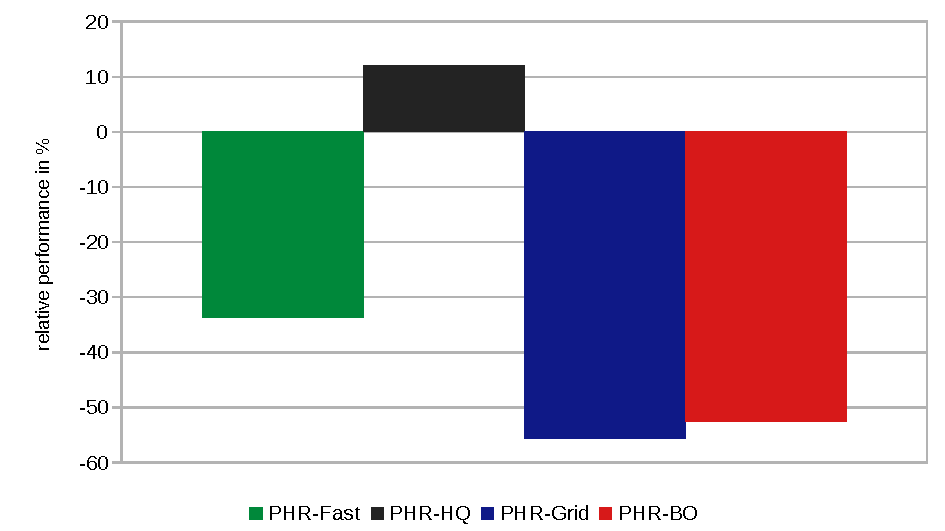
\includegraphics[width=300pt]{images/performance_difference.pdf}
    \caption{Relative difference to LBVH in percent.}
    \label{fig:difference}
\end{figure}
\subsection{Optimization Performance}
Figure \ref{fig:optimization} shows optimization times divided through average frame time, or in other words, how many frames could potentially be rendered instead of executing the optimization. Considering that the average performance increase of both methods amounted around 50\%, i.e. can potentially half the rendering time, optimizations start to become viable at half a frames duration and below. So even though the search space used in grid search is relatively low, the achieved times never reached what would be feasible in interactive applications. Bayesian optimization performed considerably better, but only reached competitive times in a few cases. Note that reaching this time does not equal a performance increase but just a hypothetical chance that frame times are increased. 

This shows that the presented optimization approaches still lack in performance and are not yet viable. PHR needs to be executed to evaluate the cost function, which is especially costly for parameters that result in high build times. This could be improved by limiting the search spacer further or making it dynamic and related to the scene's complexity. An interrupt after a maximum execution time might also be a solution. Bayesian optimization uses a costly run with maxed out parameters to determine the maximum build cost. This could be solved by reusing max values from previous optimizations. This topic is discussed further in section \ref{discussion_execute}.
\begin{figure}[H]
    \centering
    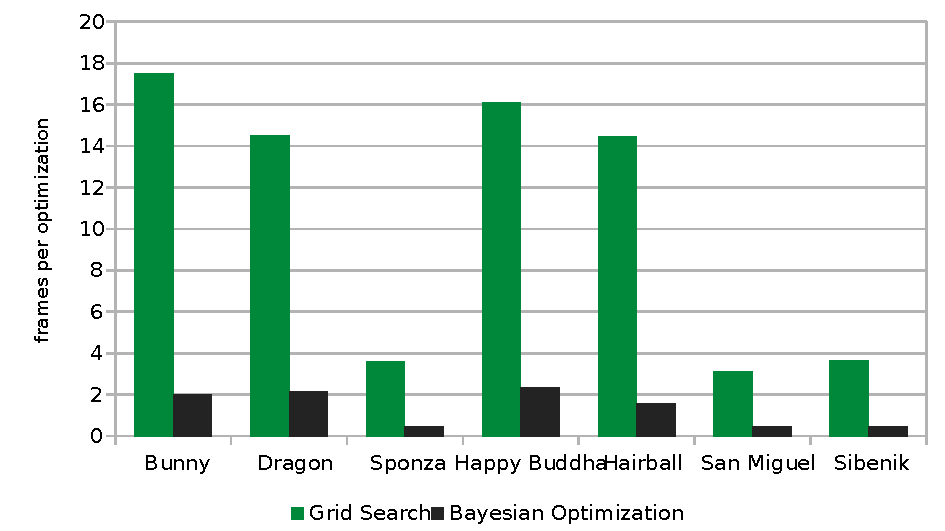
\includegraphics[width=300pt]{images/frame_per_optimization.pdf}
    \caption{Number of potential frames during optimization.}
    \label{fig:optimization}
\end{figure}
\clearpage
\begin{table}
\caption{Performance comparison of a representative selection of tested configuration at 256x256 resolution.}
\label{tab:frametime}
\centering
\begin{tabular}{ | c | m{3.5em} | m{3.5em} | m{3.5em} | m{3.5em} | m{3.5em} |  m{3.5em}|}
\hline
& build time (ms) & render time (ms) & frame time ms & build time (ms) & render time (ms) & frame time ms\\
\hline
& \multicolumn{1}{|m{4.5em}}{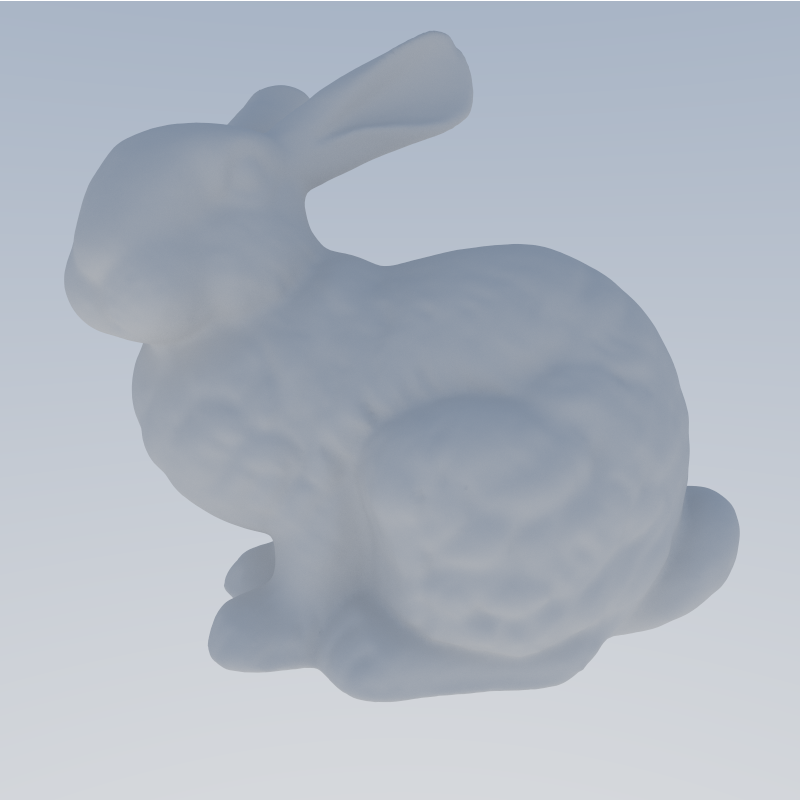
\includegraphics[width=60pt]{images/bunny.png}} &     \multicolumn{2}{m{4em}|}{Bunny \#triangles 144k} 
& \multicolumn{1}{|m{4.5em}}{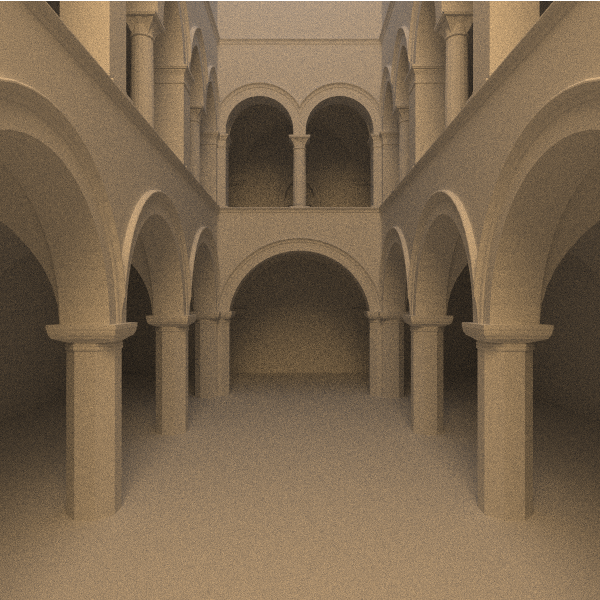
\includegraphics[width=60pt]{images/sponza.png}} & \multicolumn{2}{m{4em}|}{Sponza \#triangles 66k}\\
\hline
LBVH & 152.0 & 21.9 & 173.9            & 70.4 & 227.0 & 297.5 \\
PHR-Fast & 70.5 & 20.1 & 90.6          & 27.6 & 184 & 211.6 \\
PHR-HQ & 273.0 & 20.7 & 293.7          &  94.7 & 182 & 276.7\\
\hline
PHR-Grid & 14.4 & 20.8 & 35.2        &  17.2 & 207 & 224.2\\
PHR-BO & 14.2 & 20.7 & 34.97         &  21.7 & 200 & 221.7\\
\hline
& \multicolumn{1}{|m{4.5em}}{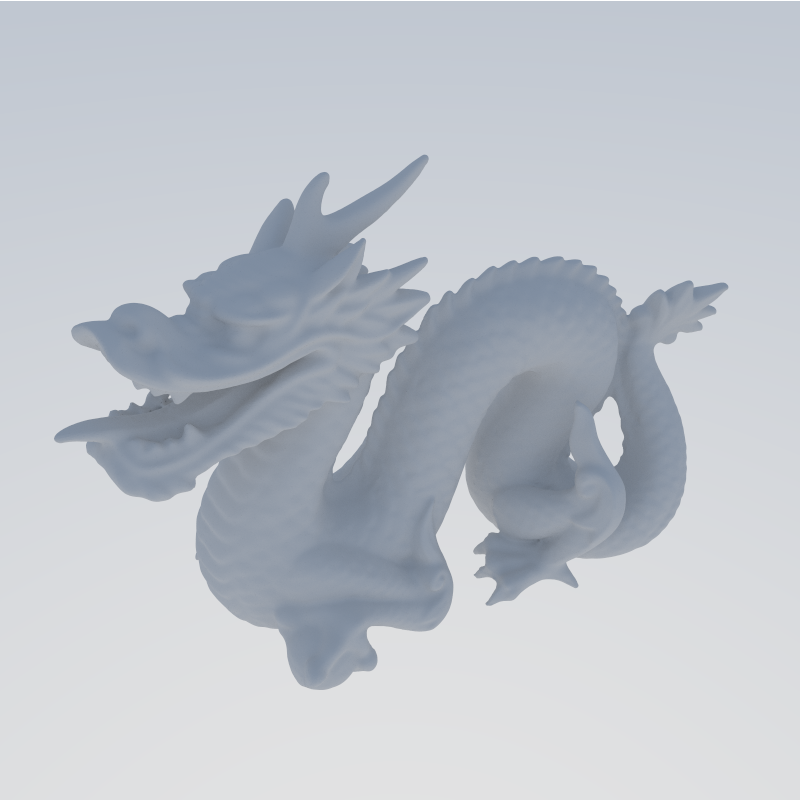
\includegraphics[width=60pt]{images/dragon.png}} &     \multicolumn{2}{m{4em}|}{Dragon \#triangles 817k}

& \multicolumn{1}{|m{4.5em}}{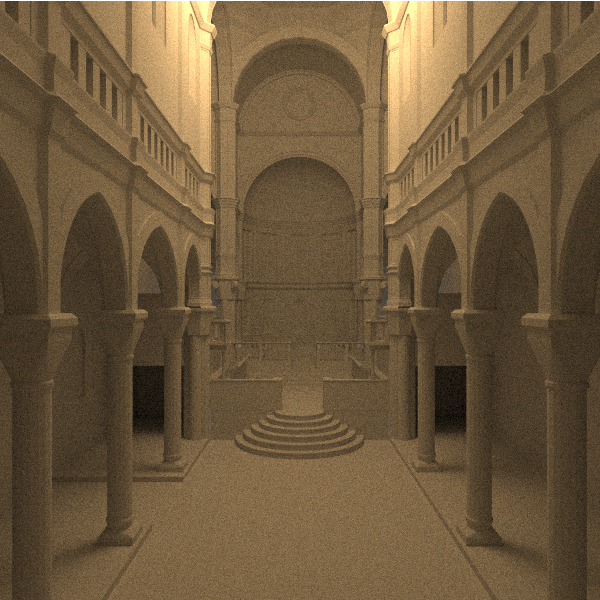
\includegraphics[width=60pt]{images/sibenik.png}} & \multicolumn{2}{m{4em}|}{Sibenik \#triangles 75k}\\

\hline
LBVH & 900.0 & 28.1 & 928.2              &  72.1 & 226.1 & 298.1\\
PHR-Fast & 150.0 & 32.5 & 182.5            &  32.5 & 205 & 237.5\\
PHR-HQ & 1090.0 & 29.0 & 1119.0              &  98.4 & 187  &285.4\\
\hline
PHR-Grid & 31.7 & 63.5 & 95.2            & 19.1 & 236 & 255.1  \\
PHR-BO & 30.8 & 66.1 & 96.9              & 28.1 & 220 & 248.1 \\
\hline
& \multicolumn{1}{|m{4.5em}}{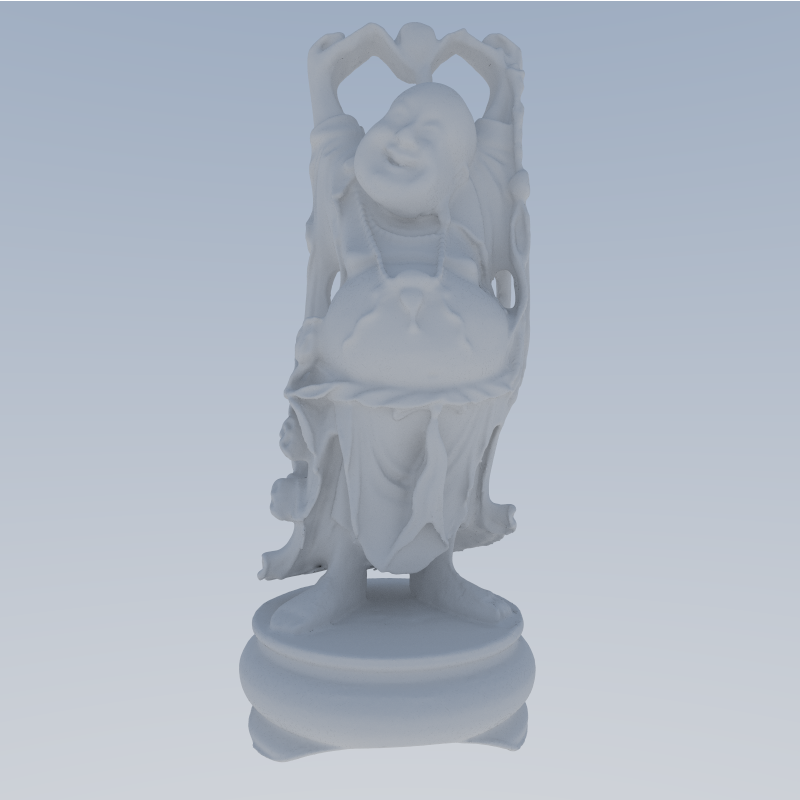
\includegraphics[width=60pt]{images/buddha.png}} & \multicolumn{2}{m{4em}|}{Happy Buddha \#triangles 1087k}

& \multicolumn{1}{|m{4.5em}}{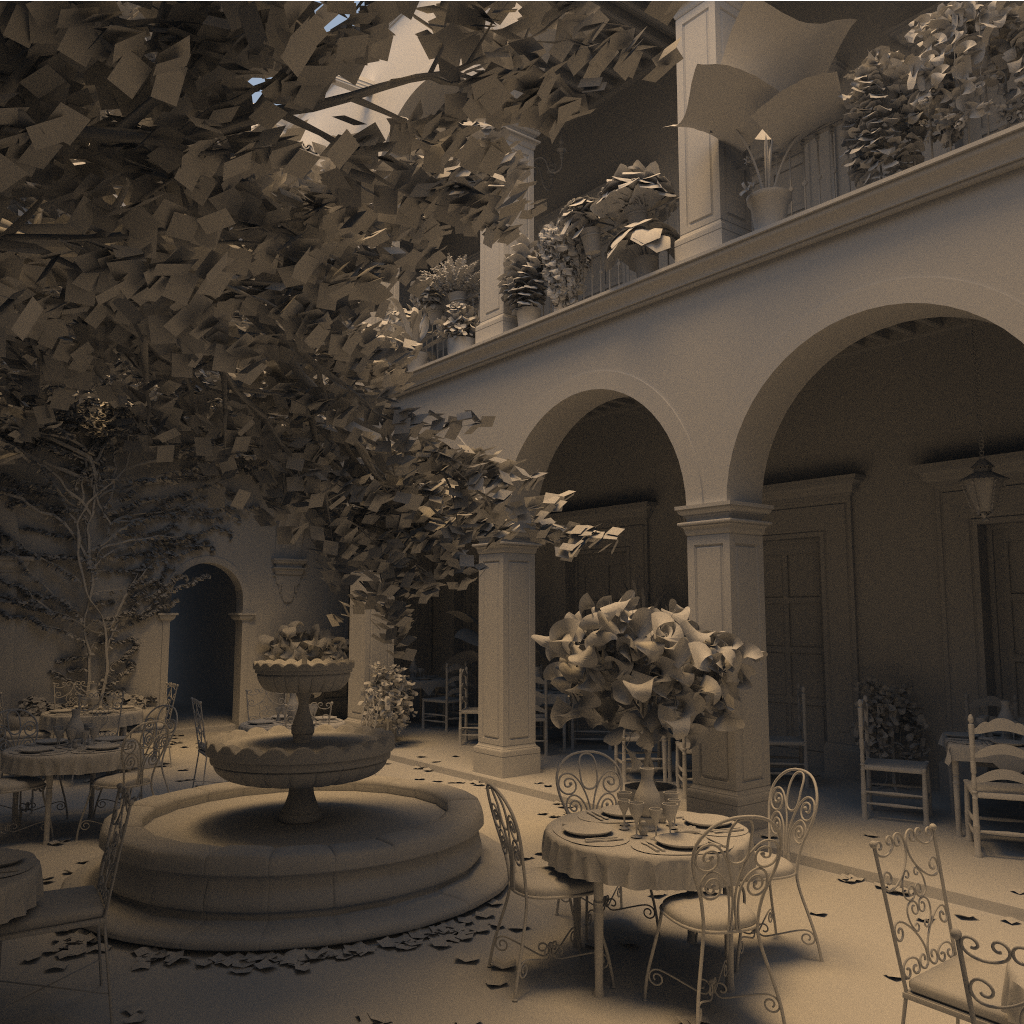
\includegraphics[width=60pt]{images/san_miguel.png}} &     \multicolumn{2}{m{4.5em}|}{San Miguel \#triangles 5617k}\\


\hline
LBVH & 1080 & 25 & 1105                    & 6010.0 & 816.0 & 6826.6 \\                   
PHR-Fast & 190 & 27.6 & 217.6                   & 432.0 & 7830.0 & 8262.0 \\
PHR-HQ & 1250 & 23.7 & 1273.7                     & 2600.0 & 812.3 & 3412.3 \\
\hline
PHR-Grid & 40.5 & 57.5 &98                   & 1300.0 & 1856.6 & 3156.6  \\
PHR-BO & 42.1 &58 &100.1                     & 815.0 & 3203.3 & 4018.3 \\
\hline
\end{tabular}
\end{table}
\cleardoublepage
\section{Discussion}


\section{Conclusion}

\subsection{Further Work}
Path tracing is a very extensive topic and especially considering the task of writing a complete path tracer, there is a lot of work left open. Considering the path tracer, a missing but essential aspect is denoising. As discussed earlier, recently a lot of progress has been achieved in that field of research and integrating some of that into this project would be an interesting addition. Importance sampling is another technique that was not considered in this work, but might improve it a decent amount. 
Staying with the main focus of this thesis, replacing LBVH with another fast BVH builder could bring interesting results. The full sweep SAH at the core of PHR is still relatively expensive and might be replacable by the more efficient binning SAH for better performance, or extended by using other cost functions like ray distribution heuristic or occlusion heuristic. Finally, optimization of PHRs hyperparameters is not ideal yet and might be improved by either using other optimization procedures, or improving the evaluation function.
\makeglossaries
\newglossaryentry{point}
{
    name=Point
    description={A point $P$ in three-dimensional space, consisting of three components x, y and z. In this thesis denoted using capital letters}
}
\newglossaryentry{vector}
{
    name=Vector
    description={A vector $v$ in three-dimensional space having a direction and a magnitude. In this thesis denoted using lower case letters}
}
\newglossaryentry{ray}
{
    name=Ray
    description={A ray is a semi-infinite line, usually in three-dimensional space. In this work the common representation using an origin $O$ and a direction $d$ is used. 
    \[P(t)=O+td\]
    Where the $O$ is some point within the scene space and the $d$ is some vector along which the ray travels in a straight line. Points along this line can be described using the distance $t$, with $P(0)=O$ and $P(1)=O+d$.}
}
\newglossaryentry{ray casting}
{
    name=Ray Casting
    description={}
}
\newglossaryentry{tree}
{
    name=Tree
    description={}
}
\newacronym{aabb}{AABB}{Axis-Aligned Bounding Box}
\newacronym{obb}{OBB}{Oriented Bounding Box}
\newacronym{bvh}{BVH}{Bounding Volume Hierarchy}
\newacronym{phr}{PHR}{Progressive Hierarchical Refinement}
\newglossaryentry{aabb}
{
    name=Axis-aligned Bounding Box
    description={}
}
\newglossaryentry{obb}
{
    name=Oriented Bounding Box
    description={}
}
\newglossaryentry{bounding sphere}
{
    name=Bounding Sphere
    description={}
}

\section{Terminology}
This section provides information and notation about terms used throughout this thesis.
\printglossary[type=\acronymtype]
\printglossary

\part*{Bibliography}
\addcontentsline{toc}{part}{Bibliography}
\nocite{*}
\bibliographystyle{apalike}
\bibliography{literatures/list}
\end{document}